\chapter{Assignment: Data Inspection}
\label{hw:data-inspection}

\newthought{Understanding the data is crucial} for any data science task. And the best way to achieve this is with visualizations. Use FTO3 data from Dr Reddy's and group them by Batch using the Pivot Table widget and its Grouped Data output.

\begin{figure}[h]
  \centering
  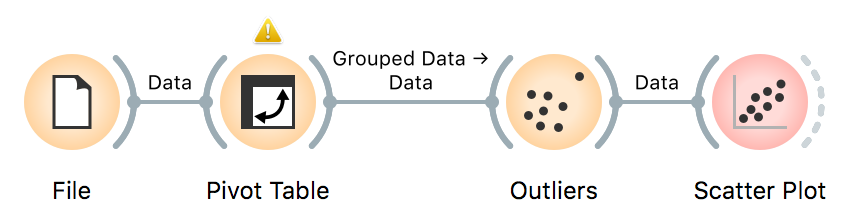
\includegraphics[width=\linewidth]{data-inspection.png}%
  \caption{Workflow for the assignment.}
  \label{fig:data-inspection-workflow}
\end{figure}

\begin{enumerate}
    \item How are the data distributed? Are there any outlying batches or do they are have a similar range of attributes?
    \item Observe the relationship between airflow (airflow…actual) and drive speed (drive.speed…actual). Is there a categorical variable that nicely splits the data?
    \item Try to find an interesting combination of attributes for Sieve Diagram. What does the combination tell you?
\end{enumerate}